\documentclass{beamer}
\beamertemplatenavigationsymbolsempty
\usecolortheme{beaver}
\setbeamertemplate{blocks}[rounded=true, shadow=true]
\setbeamertemplate{footline}[page number]
%
\usepackage[utf8]{inputenc}
\usepackage[english,russian]{babel}
\usepackage{amssymb,amsfonts,amsmath,mathtext}
\usepackage{subfig}
\usepackage{svg}
\usepackage[all]{xy} % xy package for diagrams
\usepackage{array}
\usepackage{multicol}% many columns in slide
\usepackage{hyperref}% urls
\usepackage{hhline}%tables

%----------------------------------------------------------------------------------------------------------
\title[\hbox to 56mm{Многократное обучение в рекоммендательных системах}]{Многократное обучение в рекоммендательных системах}
\author[Прозорова Л.\, И.]{Прозорова Лилия Игоревна}
\institute{}
\date{\footnotesize
\par\smallskip\emph{Руководитель:} Хританков Антон Сергеевич
\par\smallskip\emph{Консультант:} В.\,С.~Веприков
\par\bigskip\small 2024}
%----------------------------------------------------------------------------------------------------------
\begin{document}
%----------------------------------------------------------------------------------------------------------
\begin{frame}
\thispagestyle{empty}
\maketitle
\end{frame}
%----------------------------------------------------------------------------------------------------
\begin{frame}{Многократное обучение в рекоммендательных системах}
\footnotesize \textbf{Задача:} Исследовать эфффект вырождения аудитории и ассортимента товаров в рекомендательных системах с многократным обучением.
\smallskip \smallskip
\begin{columns}[c]
    \column{0.45\textwidth}
    \scriptsize \textbf{Формат данных:} Пользователи и товары описываются признаками: $C \subset \mathbb{R}^d, W \subset \mathbb{R}^l$, имеющими распределение $f_c^t$ и $f_w^t$. $u : C \times W \rightarrow [0, 1]$ - фиксированная функция полезности товара для данного пользователя.
    
    \column{0.55\textwidth}
    \scriptsize \textbf{Базовое решение:} Моделирование работы динамической системы с использованием алгоритмов Сollaborative filter, CMF, PopularityRecommender

\end{columns}
\smallskip \smallskip 
\scriptsize \textbf{Оценка вырождения:} На каждой итерации обучаем простую модель для приближения функций плотности $f_c^t$ и $f_w^t$, оцениваем невязку данной модели.
\scriptsize
% \bigskip
\begin{figure}
        \centering
        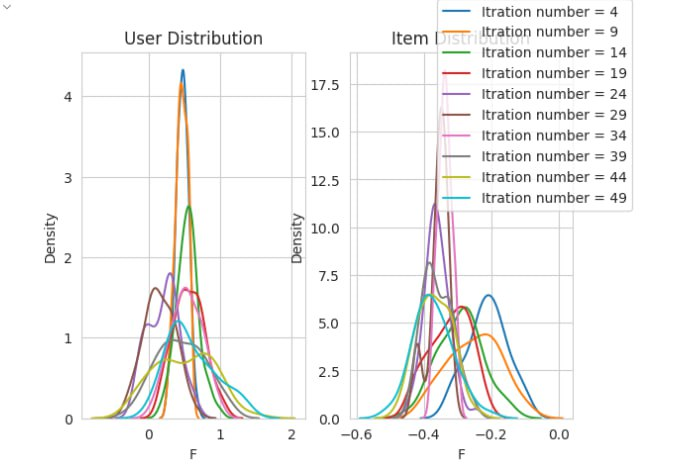
\includegraphics[width=0.50\textwidth]{distributions.jpg}
\end{figure}
% Важное {\color{red}сообщение}.
\end{frame}
%----------------------------------------------------------------------------------------------------
\end{document} 